\documentclass[12pt]{article}
\usepackage{amssymb, amsmath, amsfonts, bm, graphicx, geometry}
\usepackage{tabularx, booktabs, float, enumitem, multicol, mathtools,mathrsfs}
\geometry{margin=1in}


\title{}
\date{}
\author{}

\begin{document}

\begin{titlepage}
    \centering
    \vspace*{1in}

    % Title of the experiment and identifying number
    {\Large\bfseries Technical Memo: RC Circuit Characterization (ESC 221) \par}
    \vspace{1.5cm}

    % Course number
    {\large ESC 251 Systems Engineering\par}
    \vspace{2cm}

    % Author's name
    {\large \textbf{Authors:} Zeshui Song, Roy He \par}
    \vspace{0.5cm}


    % Name of organization sponsoring the work
    {\large Cooper Union \par}

    \vspace*{1in}
\end{titlepage}
\newpage

\section{Introduction/Background}
This technical memo investigates the time domain response of a series resistor-capacitor (RC) circuit to a square wave voltage input. The objective is to observe the charging and discharging voltage behavior across the capacitor, and analyze the relationship between the time constant of the circuit and its ability to reach a steady state value given varying input frequencies. Additionally, parametric analysis will be conducted to vary the effective resistance of the circuit (changing the time constant), and varying the frequency of the square wave voltage input.\\\\
\textbf{Experimental Method}\\\\
In the series RC circuit constructed as shown in Figure \ref{fig:Circuit}, the function generator produces a square-wave input voltage with an amplitude of 5 V and periods of 8$\tau$ and 2$\tau$, where $\tau$ is the circuit time constant. The voltage across the capacitor is measured on an oscilloscope alongside the Transistor-Transistor Logic (TTL) output of the function generator. By varying the input voltage frequency, the charging and discharging behavior of the capacitor can be observed. The physical experimental set up is shown in Figure \ref{fig:setup} and the physical circuit is shown in figure \ref{fig:realcircuit}.\\\\
Note that the TTL output of the function generator is synchronized in time with the actual voltage output, but is limited to 5 V and inverted in polarity when displayed on the oscilloscope.
\begin{figure}[H]
    \centering
    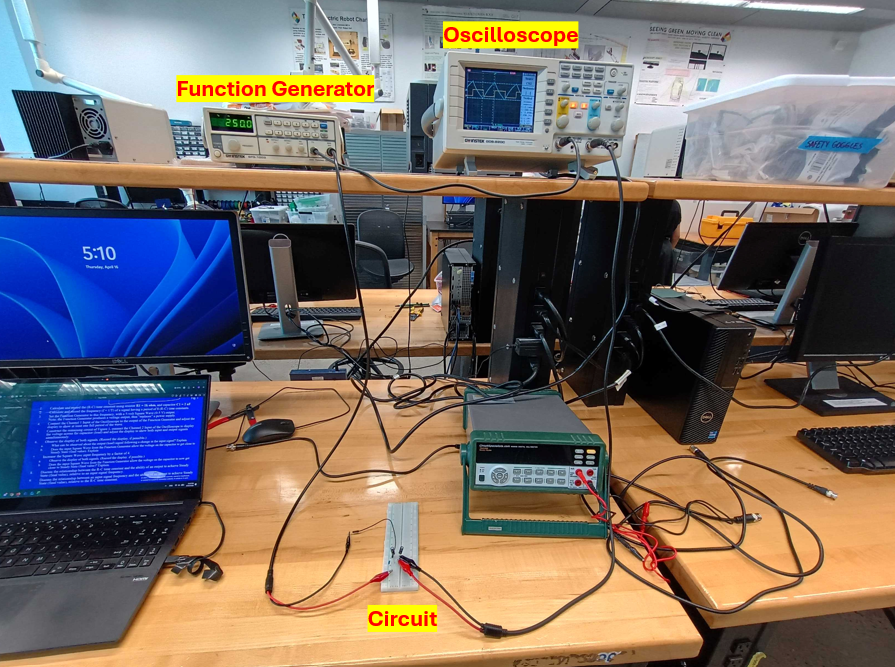
\includegraphics[width=0.6\linewidth]{set up.png}
    \caption{Physical experimental setup showing the function generator, oscilloscope, and series RC circuit. The oscilloscope probes are connected across the capacitor to measure the voltage response, and to the TTL output of the function generator for reference.}
    \label{fig:setup}
\end{figure}
\begin{figure}[H]
    \centering
    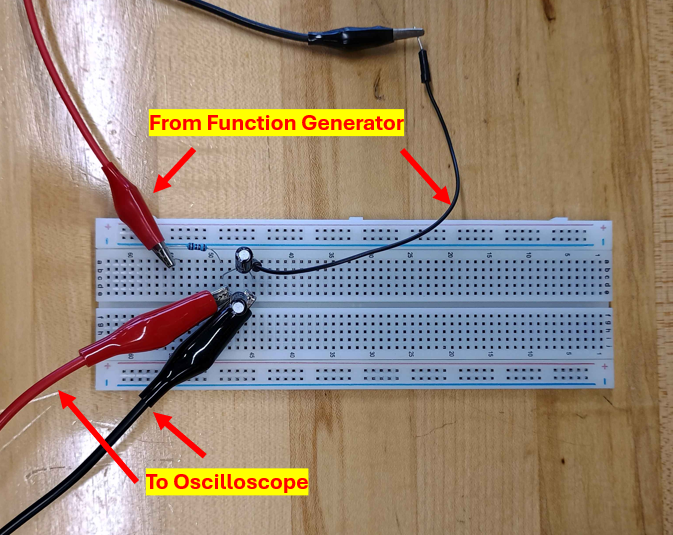
\includegraphics[width=0.6\linewidth]{real circuit.png}
    \caption{Physical breadboard circuit showing the two 1 $\mu$F capacitors wired in parallel to achieve the desired capacitance of 2 $\mu$F, and the 1 k$\Omega$ resistor. The function generator is connected to the input of the circuit, and the oscilloscope probes are connected across the capacitor for voltage measurement.}
    \label{fig:realcircuit}
\end{figure}
\section{System Model Development}
The series RC circuit can be modeled using a lumped parameter approach, where the equivalent resistance and capacitance are represented as discrete components as shown in Figure \ref{fig:Circuit}. This RC circuit is a first-order linear time-invariant (LTI) system, and its behavior can be described by a first-order ordinary differential equation (ODE) derived from Kirchhoff's current law (KCL) at node a.
\begin{figure}[H]
    \centering
    
\includegraphics[width=0.6\linewidth]{Circuit.png}
    \caption{A series RC circuit consisting of a resistor and capacitor in series with a square wave voltage input source. Nodes A and B are the measurement points for the voltage across the capacitor.}
    \label{fig:Circuit}
\end{figure}
\noindent
The governing equation for the voltage across the capacitor $v_C(t)$ is derived in Appendix 1 and is given by:
\[\boxed{RC \frac{dv_C}{dt} + v_C = v_\text{in}\quad \text{(governing eqn.)}}\]
The transfer function of the circuit is derived in Appendix 1 and is given by:
\[\boxed{G(s) = \frac{V_C(s)}{V_\text{in}(s)} = \frac{1}{RCs + 1} \quad \text{(transfer fxn.)}}\]
\textbf{Time Domain Specifications}\\
\underline{Time Constant}
\[\tau = RC = [1\times10^3\,\Omega][2\times10^{-6}\,\text{F}] = 2 \times 10^{-3} \, \text{s}\]
\[\boxed{\tau = 2 \times 10^{-3} \, \text{s}}\]
\underline{Rise Time}\\
As derived in Appendix 1, the charging voltage response of the capacitor to a step input of magnitude $v_m$ is given by:
\[v_C(t) = v_m\left(1 - e^{-t/\tau}\right)\]
Thus, the 10-90\% rise time can be calculated as follows:
\[\text{10\%:}\quad v_C(t) = 0.1 v_m = v_m\left(1 - e^{-t/\tau}\right) \implies t = 0.105\tau\]
\[\text{90\%:}\quad v_C(t) = 0.9 v_m = v_m\left(1 - e^{-t/\tau}\right) \implies t = 2.302\tau\]
\[\boxed{t_r = t_{90\%} - t_{10\%} = 2.197\tau = 4.394 \times 10^{-3} \, \text{s}}\]
\underline{Settling Time}\\
Using the 2\% criterion for settling time, we can calculate the settling time as follows:
\[\boxed{t_s = 4\tau = 8\times10^{-3}\,\text{s}}\]
\underline{DC Gain}\\
Comparing the transfer function to the standard form of a first-order system, we can identify the DC gain as follows:
\[\boxed{K = 1}\]
\underline{Pole and Stability}\\
The pole of the system is given by the root of the denominator of the transfer function:
\[RCs + 1 = 0 \implies s = -\frac{1}{RC} = -\frac{1}{\tau}\]
Since the pole is located in the left half of the complex plane, the system is stable.\\\\
\textbf{Model Assumptions}\\
The function generator is assumed to produce an ideal square wave voltage input with instantaneous transitions between 0 V and $v_m$, and a duty cycle of 50\%. The internal resistance of the function generator is assumed to be negligible compared to the 1 k$\Omega$ resistor in the circuit. The label values of the resistance and capacitance are assumed to be accurate, and the breadboard and connecting wires are assumed to have negligible resistance and capacitance.
\section{Simulation and Prediction}
It is predicted that the capacitor will follow an exponential charging and discharging curve defined by the time constant $\tau = RC$. The time domain response of the voltage is derived in Appendix 1 for each period of the square wave input voltage, and is given by:
\[\boxed{v_C(t) =
\begin{cases}
v_m\left(1 - e^{-t/\tau}\right), & t < T/2 \quad \text{(charging)}\\
v_me^{-t/\tau}\left(e^{\frac{T}{2\tau}}-1\right), & t \ge T/2\quad \text{(discharging)}
\end{cases}}\]
Thus, it is expected that when the period of the input voltage is much larger than the time constant ($T \gg \tau$), the capacitor will have sufficient time to charge and discharge fully, reaching a steady state value of $v_m$ during the charging phase and 0 V during the discharging phase. However, when the period of the input voltage is comparable to the time constant ($T \approx \tau$), the capacitor will not have sufficient time to charge and discharge fully, resulting in a voltage response that does not reach the steady state values of $v_m$ and 0 V, but rather oscillates between intermediate values.\\\\
Where the theoretical time constant is calculated to be 
\[\tau = 2 \times 10^{-3} \, \text{s}\]
The theoretical voltage response of the capacitor is plotted below in Figures \ref{fig:4tau} and \ref{fig:squarewave}:
\begin{figure}[H]
    \centering
    
\includegraphics[width=1\linewidth]{Figure_1.png}
    \caption{Theoretical capacitor voltage response to a step voltage input with period 8$\tau$, shown alongside the voltage input waveform and time constant ($\tau$) for reference. With the input turned on for $4\tau$, the capacitor is expected to reach approximately 98.2\% of its steady-state voltage during each charging interval.}
    \label{fig:4tau}
\end{figure}
\begin{figure}[H]
    \centering
    
\includegraphics[width=1\linewidth]{Figure_3.png}
    \caption{Comparison of theoretical capacitor voltage responses to square wave of varying periods (2$\tau$ and 8$\tau$), with the voltage input waveform and time constant ($\tau$) for reference.}
    \label{fig:squarewave}
\end{figure}
\section{Experimental Results}
\textbf{Input: $f=62.5$ Hz, $T=8\tau$, Pulse Duration = $4\tau$}
\begin{figure}[H]
    \centering
    
\includegraphics[width=0.6\linewidth]{1.png}
    \caption{Oscilloscope reading showing a peak capacitor voltage of 5.76V, indicating that the input voltage was miscalibrated and is approximately 5.76V rather than the expected 5V.}
    \label{fig:exp1}
\end{figure}
\begin{figure}[H]
    \centering
    
\includegraphics[width=0.6\linewidth]{1-1.png}
    \caption{The experimental time constant $\tau$ was found to be 1.9 ms, at the point where the capacitor voltage reached approximately 63.2\% of its steady-state value ($0.63\cdot[5.76\,\text{V}]$).}
    \label{fig:exp1-1}
\end{figure}
\[\boxed{\tau_\text{exp} = 1.9\times10^{-3} \, \text{s}}\]
\textbf{Input: $f=250$ Hz, $T=2\tau$, Pulse Duration = $\tau$}
\begin{figure}[H]
    \centering
    
\includegraphics[width=0.6\linewidth]{2.png}
    \caption{Oscilloscope reading of the peak voltage across the capacitor for the 2$\tau$ case to be 2.6V. Note that the minimum voltage for this case is not 0V, as the capacitor does not have sufficient time to fully discharge before the next charging interval begins.}
    \label{fig:exp2}
\end{figure}
\newpage
\noindent
\textbf{Summary of Results}
\begin{table}[h!]
\centering
\caption{Comparison of Calculated and Experimental RC Circuit Parameters}
\label{table:results_summary}
\begin{tabular}{|l|c|c|}
\hline
\textbf{Parameter} & \textbf{Theoretical Value} & \textbf{Experimental Value} \\ \hline
Time Constant ($\tau$) & 2.0 ms & 1.9 ms \\ \hline
Input Voltage ($V_m$) & 5.0 V & $\approx$ 5.76 V \\ \hline
Peak $V_C$ ($T=8\tau$) & $\approx$ 5.0 V & 5.76 V \\ \hline
$\Delta V_C$ ($T=2\tau$) & 2 V* & 2.6 V \\ \hline
\end{tabular}
\end{table}\\
*Calculated in Appendix 1. Note that if using the experimental input voltage of 5.76 V rather than the expected 5 V, the predicted $\Delta v_C$ for the 2$\tau$ case is approximately 2.304V rather than 2V.
\section{Parametric Analysis}
\textbf{Varying Effective Resistance}\\
By varying the effective resistance while keeping the capacitance and pulse duration constant, we can observe how the time constant $\tau$ affects the circuit's steady state behavior. As shown in Figure \ref{fig:param1}, decreasing the effective resistance decreases $\tau$, allowing the circuit to approach the steady state value of $v_m$ more quickly during charging and 0 V during discharging. Since the pulse duration remains constant, circuits with smaller time constants reach closer to their steady state values within each interval, while circuits with larger time constants do not fully settle before the input voltage changes again.
\begin{figure}[H]
    \centering
    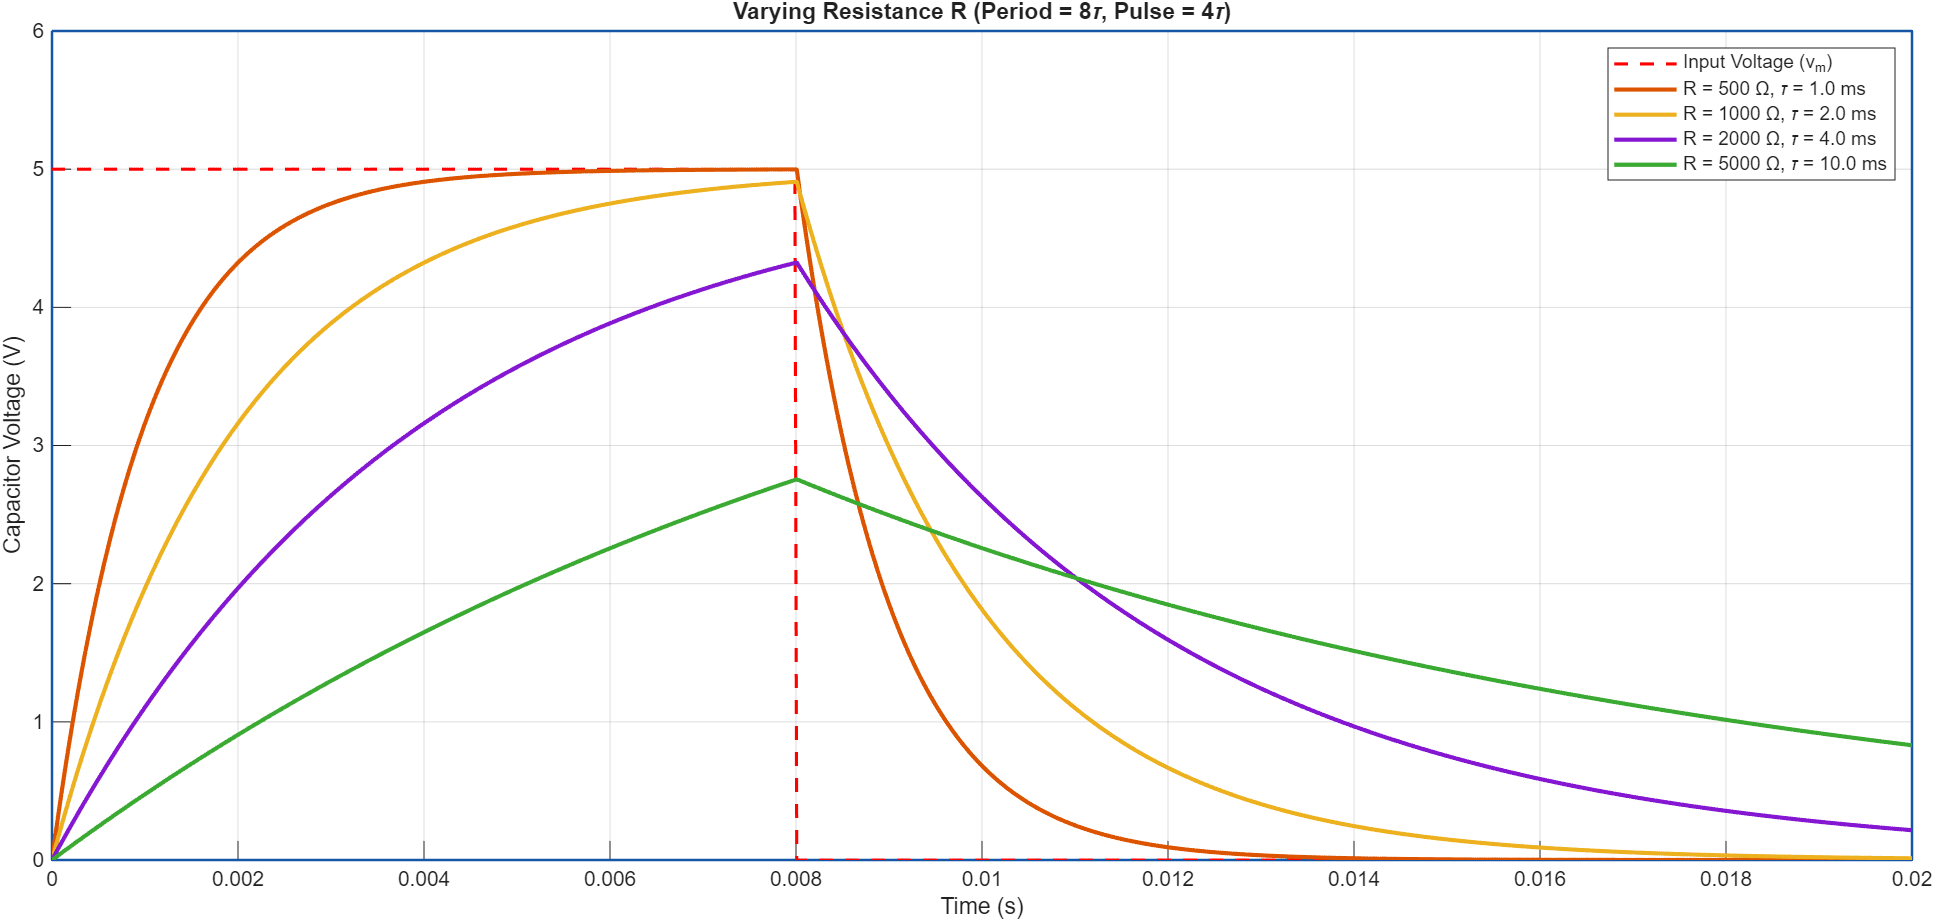
\includegraphics[width=1\linewidth]{param1.png}
    \caption{Comparison of the charging and discharging voltage responses across the capacitor for varying effective resistance values (and thus varying time constants $\tau$) with a constant \textit{absolute} pulse duration of 8 ms.}
    \label{fig:param1}
\end{figure}\noindent
\textbf{Varying Pulse Duration}\\
As discussed earlier, the relationship between the pulse duration and the time constant $\tau$ determines whether the capacitor voltage can reach steady state within each interval of the square wave input. Keeping $\tau$ fixed while varying the pulse duration produces a similar trend, as shown in Figure \ref{fig:comparison}. As the pulse duration decreases, the capacitor voltage does not have enough time to fully charge or discharge before the input voltage changes, preventing the response from reaching its steady state values.
\begin{figure}[H]
    \centering
    
\includegraphics[width=1\linewidth]{Figure_2.png}
    \caption{Comparison of theoretical capacitor voltage responses to step voltage inputs with periods of 2$\tau$ through 10$\tau$ (pulse durations of 1$\tau$ to 5$\tau$). The cases with 1$\tau$ and 4$\tau$ pulse durations are highlighted for comparison with experimental results. As the pulse duration increases, the capacitor voltage response approaches the steady-state value of $v_m$ according to the exponential charging curve.}
    \label{fig:comparison}
\end{figure}\noindent
Further analysis on Figure \ref{fig:squarewave} shows that after the transient ramp up, the max and min voltage across the capacitor for steady state oscillations are dependent on the pulse duration relative to the time constant. By plotting the max (peak) and min (trough) voltage across the capacitor for varying pulse durations in Figure \ref{fig:param2}, we can see that as the pulse duration increases, the max voltage approaches $v_m=5$ V and the min voltage approaches 0 V, following an exponential curve.
\begin{figure}[H]
    \centering
    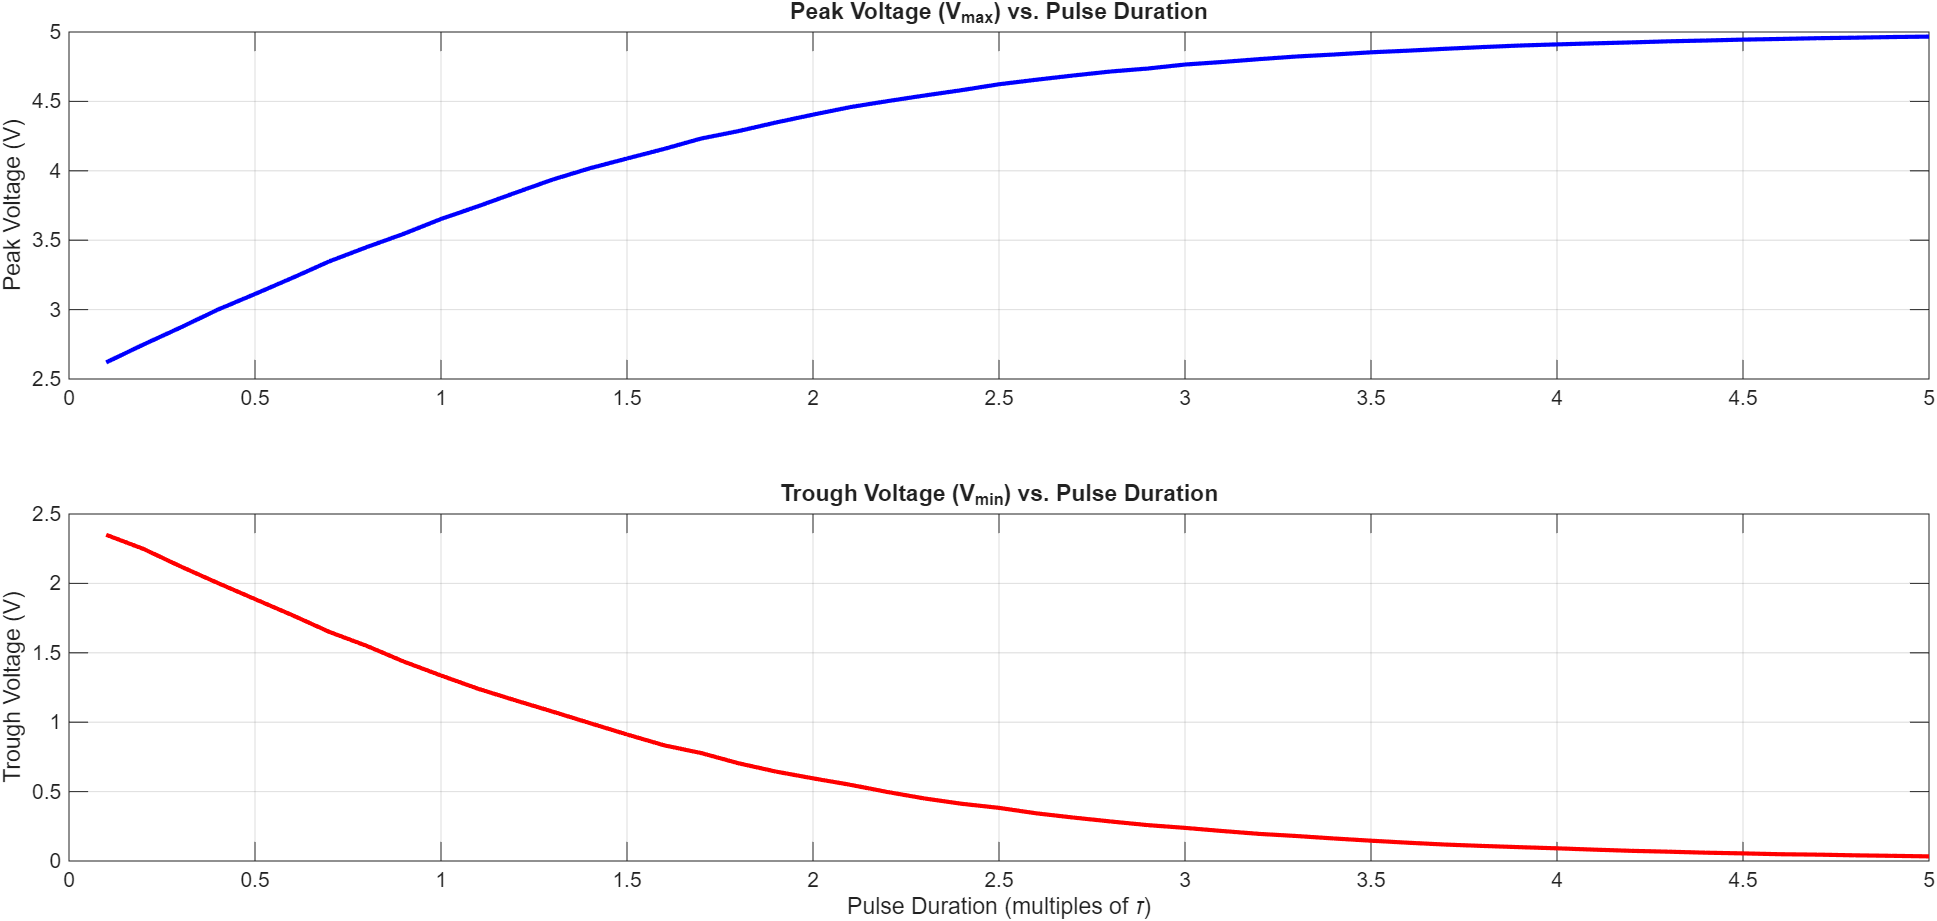
\includegraphics[width=1\linewidth]{param2.png}
    \caption{Maximum and minimum voltages across the capacitor for varying pulse durations at steady state oscillations after the transient ramp up.}
    \label{fig:param2}
\end{figure}
\section{Discussion and Future Work}
The trends observed in the experimental results are consistent with the theoretical predictions based on the model developed for the series RC circuit. There are some discrepancies between the theoretical and experimental values, such as the miscalibrated input voltage and the slightly smaller experimental time constant, which is a result of non-ideal behavior of the components and setup errors.\\\\
For future work, it would be interesting to explore the effects of sinusoidal voltage inputs to see the AC response of the circuit, and to further analyze the frequency response of the system. Additionally, we could better model the system by including the internal resistance of the function generator and the oscilloscope to get a more accurate prediction of the time constant and voltage response.
\newpage
\section*{Appendix 1: Derivations and Calculations}
\textbf{Transfer Function Derivation}
\begin{center}
    
\includegraphics[width=0.6\linewidth]{Circuit.png}
\end{center}
Defining the input voltage as $v_\text{in}(t)$ and the output voltage across the capacitor as $v_C(t)$, the governing equation for the circuit can be derived using Kirchhoff's current law (KCL) at node a, using node b as the reference node:
\[\frac{v_\text{in}-v_a}{R} = C\frac{dv_C}{dt}\]
Since $v_a = v_C$, the governing equation can be rewritten as:
\[\boxed{RC \frac{dv_C}{dt} + v_C = v_\text{in}\quad \text{(governing eqn.)}}\]
Taking the Laplace transform, assuming zero initial conditions:
\[RCsV_C(s) + V_C(s) = V_\text{in}(s)\]
\[\boxed{G(s) = \frac{V_C(s)}{V_\text{in}(s)} = \frac{1}{RCs + 1} \quad \text{(transfer fxn.)}}\]
\textbf{Calculation for Predicted Voltage Response (for a single step input)}\\
Defining the following parameters:
\begin{itemize}
    \item $v_m$: Amplitude of the square wave input voltage
    \item $T$: Period of the square wave input voltage
\end{itemize}
The function generator has a duty cycle of 50\%, meaning that it is on for half of each period ($T/2$). Thus, one period of the square wave input voltage can be defined using the Heaviside step function $\mathscr{U}(t-a)$ as follows:
\[v_\text{in}(t)=v_m(1-\mathscr{U}(t-T/2))\]
Such that
\[v_{\text{in}}(t) = 
\begin{cases} 
v_m, & t < T/2 \\
0, & t \ge T/2 
\end{cases}\]
Using the governing equation derived above:
\[RC\frac{dv_C}{dt} + v_C = v_m(1-\mathscr{U}(t-T/2))\]
\underline{Finding $v_C(t)$}\\
Letting $\tau = RC$, the governing equation can be rewritten as:
\[\tau\frac{dv_C}{dt} + v_C = v_m(1-\mathscr{U}(t-T/2))\]
Taking the Laplace transform, assuming zero initial conditions:
\[\tau sV_C(s) + V_C(s) = v_m\left(\frac{1}{s} - \frac{e^{-\frac{T}{2}s}}{s}\right)\]
\[V_C(s) \left(\tau s + 1\right) = v_m \left(\frac{1-e^{-\frac{T}{2}s}}{s}\right)\]
\[V_C(s) = v_m(1-e^{-\frac{T}{2}s})\left(\frac{1}{s(\tau s + 1)}\right)=v_m(1-e^{-\frac{T}{2}s})\left(\frac{1/\tau}{s(s + 1/\tau)}\right)\]
Partial fraction decomposition:
\[\frac{1/\tau}{s(s + 1/\tau)} = \frac{A}{s} + \frac{B}{s + 1/\tau}\]
Using the limit method to solve for $A$ and $B$:
\[A = \lim_{s\to 0} \left(s\frac{1/\tau}{s(s + 1/\tau)} \right)= 1\]
\[B = \lim_{s\to -1/\tau} \left((s + 1/\tau)\frac{1/\tau}{s(s + 1/\tau)} \right)= -1\]
Thus, the partial fraction decomposition can be rewritten as:
\[\frac{1/\tau}{s(s + 1/\tau)} = \frac{1}{s} - \frac{1}{s + 1/\tau}\]
Plugging this back into the expression for $V_C(s)$:
\[V_C(s) = v_m(1-e^{-\frac{T}{2}s})\left(\frac{1}{s} - \frac{1}{s + 1/\tau}\right)\]
\[V_C(s) = v_m\left(\frac{1}{s} - \frac{1}{s + 1/\tau}\right)-v_m e^{-\frac{T}{2}s}\left(\frac{1}{s} - \frac{1}{s + 1/\tau}\right)\]
Taking the inverse Laplace transform:
\[v_C(t) = v_m\left(1 - e^{-t/\tau}\right) - v_m \mathscr{U}(t-T/2)\left(1 - e^{-\left(t-\frac{T}{2}\right)/\tau}\right)\]
\[\boxed{v_C(t) =
\begin{cases}
v_m\left(1 - e^{-t/\tau}\right), & t < T/2 \quad \text{(charging)}\\
v_me^{-t/\tau}\left(e^{\frac{T}{2\tau}}-1\right), & t \ge T/2\quad \text{(discharging)}
\end{cases}}\]
\newpage\noindent
\textbf{Calculation for $\Delta v_C$}\\
Input: $v_m = 5$ V, $f=250$ Hz, $T=2\tau$, Pulse Duration = $\tau$\\\\
Max voltage is at $t=T/2 = \tau$:
\[v_C(\tau) = v_m\left(1 - e^{-\tau/\tau}\right) = v_m\left(1 - e^{-1}\right) \approx 0.63v_m\]
Minimum voltage is at $t=T = 2\tau$:
\[v_C(2\tau) = v_me^{-2\tau/\tau}\left(e^{\frac{2\tau}{2\tau}}-1\right) = v_me^{-2}\left(e^{1}-1\right) \approx 0.23v_m\]
Thus, the change in voltage across the capacitor is calculated to be:
\[\Delta v_C = v_C(\tau) - v_C(2\tau) \approx 0.63v_m - 0.23v_m = 0.40v_m = 2 \, \text{V}\]
Note that since the input voltage was miscalibrated to be approximately 5.76V rather than the expected 5 V, the predicted $\Delta v_C$ for the 2$\tau$ case is approximately 2.304V rather than 2V.
\section*{Appendix 2: Experimental Procedure}
Constructing the Circuit
\begin{enumerate}
    \item The circuit was constructed as shown in Figure \ref{fig:Circuit}, with two 1 $\mu$F capacitors wired in parallel to achieve the desired capacitance of 2 $\mu$F, and a 1 k$\Omega$ resistor. 
    \item The function generator output was set to a 5V square with the calculated frequency of 62.5 Hz for the 8$\tau$ case, and 250 Hz for the 2$\tau$ case.
\end{enumerate}
Measurement and Data Collection
\begin{enumerate}
    \item Channel 1 of the oscilloscope was connected to the TTL output of the function generator.
    \item Channel 2 of the oscilloscope was connected across the capacitor at nodes A and B to measure the voltage response.
    \item Starting with the function generator set to 62.5 Hz ($T = 8\tau$), the voltage response across the capacitor was observed and recorded on the oscilloscope.
    \item The frequency of the function generator was then changed to 250 Hz ($T = 2\tau$), and the voltage response across the capacitor was again observed and recorded on the oscilloscope.
\end{enumerate}
\section*{Appendix 3: MATLAB Code for Simulation and Parametric Analysis}
\textbf{MATLAB Code for Generating Figures \ref{fig:4tau}, \ref{fig:comparison}, and \ref{fig:param2}}
\begin{verbatim}
    close all;
clc;
clear;

% --- Common Parameters ---
r1 = 1000; 
c1 = 2e-6;
tau = r1 * c1; % Time constant
vC0 = 0;
vm = 5;
t = linspace(0, 0.02, 1000); 

% System Definition (Transfer Function)
num = 1;
den = [tau 1];
sys = tf(num, den);

%% Plot 1: Standard 4-Tau Pulse
figure(1);
T4 = 4 * tau; 
vs4 = vm * (t <= T4); 
[vC4, t_out4] = lsim(sys, vs4, t, vC0);

plot(t_out4, vC4, 'b', 'LineWidth', 2);
hold on;
plot(t, vs4, '--r', 'LineWidth', 1.5);

xline(tau, '--', 'Color', [0 0.5 0], 'Label', '\tau', ...
    'LineWidth', 2, 'LabelVerticalAlignment', 'bottom');

grid on;
xlabel('Time (s)');
ylabel('Voltage (V)');
legend('Capacitor Voltage (v_C)', 'Input Voltage (v_m)', 'Time Constant (\tau)');
title('RC Circuit Response (Period = 8\tau, Pulse = 4\tau)');
ylim([0 6]);

%% Plot 2: Shared Plot (Comparison of 1\tau through 5\tau)
figure(2);
hold on;
grid on;

% Define colors
colors = lines(5); 

for n = 1:5
    T_pulse = n * tau;
    vs_loop = vm * (t <= T_pulse);
    [vC_loop, t_out_loop] = lsim(sys, vs_loop, t, vC0);
    
    % Solid for 1 and 4, Dotted for others
    if n == 1 || n == 4
        style = '-';
        width = 2.5; 
    else
        style = ':';
        width = 1.5;
    end
    
    plot(t_out_loop, vC_loop, style, 'Color', colors(n,:), 'LineWidth', width, ...
        'DisplayName', [num2str(n), '\tau Pulse']);
end

xline(tau, '--', 'Color', [0 0.5 0], 'LineWidth', 2, ...
    'Label', '\tau', 'LabelVerticalAlignment', 'bottom', ...
    'HandleVisibility', 'off');

% Horizontal line for Max Input Voltage
yline(vm, '--k', 'Max Input (5V)', 'LineWidth', 1, ...
    'LabelHorizontalAlignment', 'right', 'HandleVisibility', 'off');

% Formatting
xlabel('Time (s)');
ylabel('Voltage (V)');
title('Comparison of RC Circuit Responses for Different Pulse Durations');
legend('Location', 'northeastoutside');
ylim([0 6]);
hold off;

%% Plot 3: Parametric Analysis (Varying Resistance R)
figure(3);
hold on; 
grid on;

R_values = [500, 1000, 2000, 5000]; % Parametric variation of Resistance
T_sim = 0.02; 
t_param = linspace(0, T_sim, 1000);
T_pulse_param = T4; % 4*tau pulse duration

vs_param = vm * (t_param <= T_pulse_param);
plot(t_param, vs_param, '--r', 'LineWidth', 1.5, 'DisplayName', 'Input Voltage (v_m)');

for R = R_values
    current_tau = R * c1; % Recalculate tau for each R 
    
    % Define specific Transfer Function for this R
    sys_param = tf(1, [current_tau 1]);
    
    % Simulate Response
    [vC_param, t_out_param] = lsim(sys_param, vs_param, t_param, vC0);
    
    % Plot with R and Tau in the legend
    plot(t_out_param , vC_param, 'LineWidth', 2, ...
        'DisplayName', sprintf('R = %d \\Omega, \\tau = %.1f ms', R, current_tau*1000));
end

% Formatting
xlabel('Time (s)');
ylabel('Capacitor Voltage (V)');
title('Varying Resistance R (Period = 8\tau, Pulse = 4\tau)');
legend('show', 'Location', 'northeast');
ylim([0 6]);
hold off;
\end{verbatim}
\textbf{MATLAB Code for Generating Figures \ref{fig:squarewave} and \ref{fig:param1}}
\begin{verbatim}
close all;
clc;
clear;

% --- Parameters ---
r1 = 1000; 
c1 = 2e-6;      % Updated to 2uF
tau = r1 * c1;  % Time constant (0.002s)
vC0 = 0;
vm = 5;         % Updated to 5V

% System Definition (Transfer Function)
num = 1;
den = [tau 1];
sys = tf(num, den);

% Time vector
t = linspace(0, 0.02, 5000); 

figure;

%% Subplot 1: Square Wave with Pulse Width = 1*tau
k1 = 1;
half_period1 = k1 * tau;
period1 = 2 * half_period1;
vs1 = vm * (mod(t, period1) < half_period1);

[vC1, t_out1] = lsim(sys, vs1, t, vC0);

subplot(2, 1, 1);
plot(t_out1, vC1, 'b', 'LineWidth', 2);
hold on;
plot(t, vs1, '--r', 'LineWidth', 1.5);

xline(tau, '--', 'Color', [0 0.5 0], 'Label', '\tau', ...
    'LineWidth', 2, 'LabelVerticalAlignment', 'bottom');

grid on;
ylim([0 6]);
ylabel('Voltage (V)');
legend('v_C', 'v_m', '\tau');
title(['Square Wave Response: Period = 2\tau, Pulse Width = \tau']);

%% Subplot 2: Square Wave with Pulse Width = 4*tau
k2 = 4;
half_period2 = k2 * tau;
period2 = 2 * half_period2;
vs2 = vm * (mod(t, period2) < half_period2);

[vC2, t_out2] = lsim(sys, vs2, t, vC0);

subplot(2, 1, 2);
plot(t_out2, vC2, 'b', 'LineWidth', 2);
hold on;
plot(t, vs2, '--r', 'LineWidth', 1.5);

xline(tau, '--', 'Color', [0 0.5 0], 'Label', '\tau', ...
    'LineWidth', 2, 'LabelVerticalAlignment', 'bottom');

grid on;
ylim([0 6]);
xlabel('Time (s)');
ylabel('Voltage (V)');
title(['Square Wave Response: Period = 8\tau, Pulse Width = 4\tau']);

%% Figure 2: Peak and Trough Analysis vs. Pulse Duration
figure(2);

% Pulse durations from 0.1*tau to 5*tau
pulse_durations = linspace(0.1*tau, 5*tau, 50);
V_peaks = zeros(size(pulse_durations));
V_troughs = zeros(size(pulse_durations));

for i = 1:length(pulse_durations)
    T_p = pulse_durations(i);
    T_total = 2 * T_p; % 50% duty cycle
    
    % Simulate enough cycles to reach steady-state oscillation
    t_sim = linspace(0, 10*T_p + 5*tau, 2000); 
    vs_sim = vm * (mod(t_sim, T_total) < T_p);
    [vC_sim, ~] = lsim(sys, vs_sim, t_sim, vC0);
    
    % Capture peak and trough from the last full cycle
    V_peaks(i) = max(vC_sim(end-500:end));
    V_troughs(i) = min(vC_sim(end-500:end));
end

% Plot Peak Voltages
subplot(2,1,1);
plot(pulse_durations/tau, V_peaks, 'b', 'LineWidth', 2);
hold on;
grid on;
title('Peak Voltage (V_{max}) vs. Pulse Duration');
ylabel('Peak Voltage (V)');

% Plot Trough Voltages
subplot(2,1,2);
plot(pulse_durations/tau, V_troughs, 'r', 'LineWidth', 2);
hold on;
grid on;
title('Trough Voltage (V_{min}) vs. Pulse Duration');
xlabel('Pulse Duration (multiples of \tau)');
ylabel('Trough Voltage (V)');
\end{verbatim}
\section*{Appendix 4: Teammate Contributions}
\begin{itemize}
    \item Zeshui Song: Circuit construction, data collection, model development and analysis, and technical memo writing.
    \item Roy He: Circuit construction, data collection, MATLAB simulation and parametric analysis, and presentation slideshow.
\end{itemize}
\end{document}